\documentclass[kravspec/krav.tex]{subfiles}

\begin{document}

\section{Översikt av systemet}
Här beskriver vi produkten övergripande samt 
\begin{figure}[h]
    \centering
    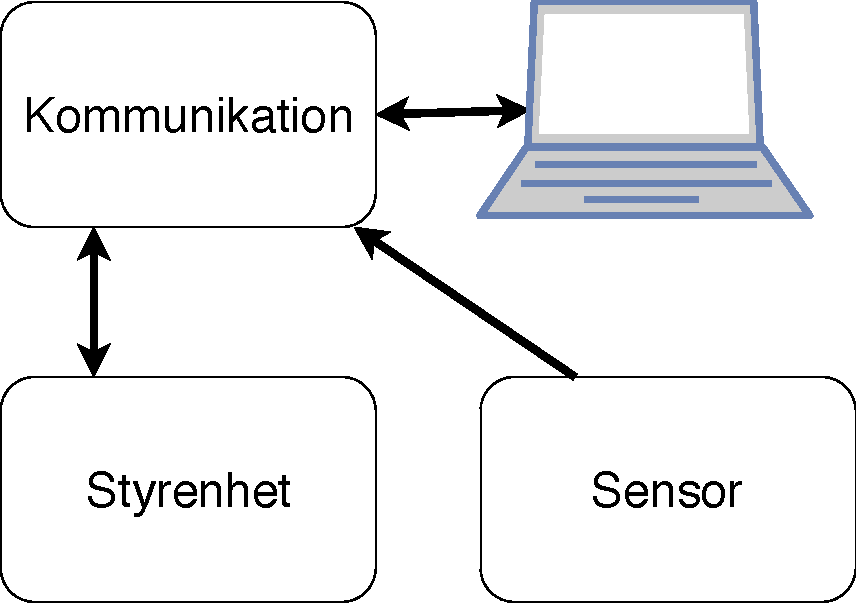
\includegraphics[width=0.6\linewidth]{kravspec/figures/overview-schema.pdf}
    \caption{Grov blockschema över moduler i produkten}
    \label{fig:overview}
\end{figure}

\subsection{Grov beskrivning av produkten}
Produkten är en bil med fyra hjul som ska med hjälp av ett känt vägnät ta sig
till en passagerare och skjutsa passageraren till önskad destination. Denna
taxibil ska kunna åka framåt, bakåt, svänga vänster och höger.  Bland annat ska
man kunna initiera en bluetooth-länk mellan bilen och en dator som har stöd för
bluetooth. Bilen ska ha ett läge där man kan fjärrstyra bilen och ett läge där
bilen ska köra autonomt i vägnätet samt undvika hinder.

\subsection{Produktkomponenter}
Lämplig hårdvara med kompletterande mjukvara kommer finnas i den kompletta
produkten. Bland annat ska även tekniskt dokumenation ingå i produkten.

\subsection{Beroenden till andra system}
Fjärstyrning av bilen skall vara beroende av en dator som har stöd för bluetooth.
Autonoma läget aktiveras från användargränsnittet tillgänglig på datorn med
bluetooth.

\subsection{Ingående delsystem}
Systemet kommer bestå av följande delsystem enligt figur
\ref{fig:overview}; Sensormodulen ska hämta data om omgivningen, bland annat
en kamera som tar bilder av vad som är framifrån, en sensor som mäter avstånd
till objekt i omgivning och tejpföljare som sensorer. Lämplig data av omgivning
skickas till kommunikationsmodell. Produkten har även en styrmodul som ser till
att bilen kan styras beroende på data från kommunikationsmodul.

\subsection{Avgränsningar}
Små väghinder som grova vägkanter och gropar tas ej hänsyn till. Vägen
förväntas bestå av hinder som är i lämplig höjd för att enhetens sensorer ska
upptäcka dem. Vägen antas vara plan utan gropar.

\subsection{Generella krav på hela systemet}

\begin{reqlist}
    \req{Bilen ska kunna skicka aktuell mätdata till den bärbara datorn.
    Mätdata inkluderar avstånd till vägkant, avstånd till hinder, avlagd
    sträcka, styrbeslut och motorernas styrning.}
    \req{Successiv inmatning av reglerparametrarna skall vara möjlig (inmatning
    utan ny kompilering}
    \req{Mätdatan skall presenteras på datorns skärm på ett användarvänligt
    sätt.}
    \req{Användaren skall kunna växla mellan autonom och manuell körning på
    bilen utan att koden ska behöva kompileras om.}
    \req{Bilen skall via fjärrstyrning (manuell körning)  kunna köra framåt,
    bakåt, stanna och svänga vänster eller höger.}
    \req{Bilen skall ha en kamera som tar bilder åtminstone åt en riktning }
    \req{Under autonom körning ska taxin kunna köra från en punkt till en annan
    i ett känt tvåfiligt vägnät.}
    \req{Under autonom körning skall bilen navigera vägnätet enligt
    högertrafik.}
    \req{Under autonom körning skall bilen stanna ifall hinder befinner sig på
    vägen.}
    \reqspec{original}{2}{Om ett hinder blockerar taxins körfält under autonom
    körning skall taxibilen köra runt objektet genom att köra i det andra
    körfältet.}
    \req{Under autonom körning skall bilen navigera genom vägnätet från en
    förutsatt positioner till en annan förutsatt destination, via kortaste
    väg.}
    \req{Bilen skall kunna stanna vid en stopplinje}
    \req{Bilen skall kunna svänga av in i en parkeringsficka och stanna där.}
    \req{Bilen skall klara av att navigera i rondeller där högertrafik gäller.}
    \reqspec{original}{2}{Bilen skall kunna delta i en tävling där tiden för
    varje uppdrag mäts.}
    \reqspec{original}{3}{Bilen skall aktivera blinkers vid svängning samt
    hämtning och avlämning.}
    \req{Bilen ska vara moduluppbyggd där varje modul innehåller en egen
    processor. En kommunikationsmodul, en styrmodul samt en sensormodul skall
    ingå.}
    \req{En karta skall kunna skickas från en bärbar dator till bilen.}
    \req{Under körning skall positionsdata fortlöpande skickas till en bärbar
    dator och visas på en karta.}
    \reqspec{original}{2}{Direktsändning av kamerabilden skall visas på en
    bärbar dator.}
    \req{Bilen ska använda sig av en styralgoritm så att den föredrar att
    befinna sig centralt i filen.}

\end{reqlist}

\end{document}
